% Image Processing Lab -- CSE220 Signals and Systems Sessional, Dept. of CSE, BUET
%
% Build:    latexmk -xelatex slides.tex
% Figures:  .venv/bin/python presentation/make_figures.py   (run from the repo root)
%
% Layout follows ref.tex (Metropolis). Every image in figures/ is real output of
% src/backend on the three photos next to this file (cat_soldier, blue_flower,
% casette); the numbers on the slides are the ones make_figures.py prints.

\documentclass[9pt,aspectratio=169]{beamer}

%================================================
% Theme
%================================================
\usetheme[numbering=fraction,progressbar=frametitle]{metropolis}
\metroset{block=fill}

\usepackage{iftex}
\ifPDFTeX\else
  % Fira ships with TeX Live; loading it by file name means XeLaTeX finds it
  % even where it is not installed as a system font
  \setsansfont{FiraSans}[Extension=.otf, UprightFont=*-Light, ItalicFont=*-LightItalic,
                         BoldFont=*-Regular, BoldItalicFont=*-Italic]
  \setmonofont{FiraMono}[Extension=.otf, UprightFont=*-Regular, BoldFont=*-Medium, Scale=0.92]
\fi

%================================================
% Packages
%================================================
\usepackage{amsmath,amssymb}
\usepackage{booktabs}
\usepackage{listings}
\usepackage{tikz}
\usetikzlibrary{positioning,arrows.meta,calc}
\graphicspath{{figures/}}

%================================================
% Colors
%================================================
\definecolor{royalblue}{HTML}{63223c}
\definecolor{seagreen}{HTML}{2E8B57}
\definecolor{custom1}{HTML}{9c596a}
\colorlet{accent}{royalblue}   % <-- switch here: royalblue | seagreen
% title bar: the accent darkened a little, so white text stays readable on it.
% Any colour works here, e.g. {accent}, {custom1}, {black!80}
\colorlet{titlebar}{accent!80!black}

\definecolor{softgray}{HTML}{F4F6F8}
\colorlet{muted}{black!55}

\setbeamercolor{frametitle}{fg=white, bg=titlebar}
\setbeamercolor{progress bar}{fg=accent, bg=accent!18}
\setbeamercolor{alerted text}{fg=accent}
\setbeamercolor{block title}{fg=white, bg=accent}
\setbeamercolor{block body}{fg=black, bg=softgray}
\setbeamercolor{standout}{fg=white, bg=accent}

%================================================
% Code style (ref.tex's, with quiet highlighting)
%================================================
\lstdefinestyle{code}{
  language=Python,
  basicstyle=\ttfamily\footnotesize,
  keywordstyle=\color{accent},
  commentstyle=\color{black!45},
  stringstyle=\color{black!70},
  backgroundcolor=\color{black!3},
  frame=single, rulecolor=\color{black!15},
  framesep=5pt, xleftmargin=5pt, xrightmargin=5pt,
  aboveskip=0pt, belowskip=0pt,
  columns=fullflexible, keepspaces=true, showstringspaces=false, breaklines=true,
}
\lstset{style=code}

%================================================
% Small helper commands
%================================================
% the Signals & Systems idea a slide is about, as a quiet line under the title
\newcommand{\concept}[1]{{\small\color{accent}\textbf{Signals \& Systems}\quad
  \color{black!70}#1}\par\medskip}
% an image with a short caption under it: \pic{height}{file}{caption}
\newcommand{\pic}[3]{\begin{tabular}[t]{@{}c@{}}%
  \includegraphics[height=#1]{#2}\\[1pt]{\footnotesize\color{muted}#3}\end{tabular}}
% one cell of the operations grid: \op{file}{name}{idea}
\newcommand{\op}[3]{\begin{minipage}[t]{2.2cm}\centering
  \includegraphics[height=2.1cm]{#1}\\[3pt]
  {\small #2}\\[-1pt]{\footnotesize\color{muted}#3}\end{minipage}}
% a blur result with its kernel (the impulse response) beside it: \kpair{kind}{caption}
\newcommand{\kpair}[2]{\begin{tabular}[t]{@{}c@{}}%
  \raisebox{0.45cm}{\includegraphics[height=0.8cm]{kernel_#1}}\,%
  \includegraphics[height=1.7cm]{blur_#1}\\[1pt]{\footnotesize\color{muted}#2}\end{tabular}}
\newcommand{\tagline}[1]{\begin{center}\alert{#1}\end{center}}
% nearest-neighbour resize of one row, drawn as the code does it: each new
% pixel's centre (dot) points up to the old pixel under it, and the old pixels
% that get read are shaded. Positions come from (i + 1/2) * old/new, not by hand.
% \resizemap{old count}{new count}{cm per old pixel}{title}{effect}
\newcommand{\resizemap}[5]{%
\begin{tikzpicture}[x=#3cm, y=1cm, font=\footnotesize]
  \pgfmathsetmacro{\rmS}{#1/#2}
  \pgfmathtruncatemacro{\rmOld}{#1 - 1}
  \pgfmathtruncatemacro{\rmNew}{#2 - 1}
  \foreach \i in {0,...,\rmNew} {
    \pgfmathsetmacro{\p}{(\i + 0.5) * \rmS}
    \pgfmathtruncatemacro{\j}{floor(\p)}
    \fill[accent!15] (\j, 0.95) rectangle ++(1, 0.42);
  }
  \foreach \j in {0,...,\rmOld} {
    \draw[black!35] (\j, 0.95) rectangle ++(1, 0.42);
    \node[black!70] at (\j + 0.5, 1.16) {\j};
  }
  \foreach \i in {0,...,\rmNew}
    \draw[black!35] (\i * \rmS, 0) rectangle ++(\rmS, 0.42);
  \foreach \i in {0,...,\rmNew} {
    \pgfmathsetmacro{\p}{(\i + 0.5) * \rmS}
    \draw[-{Stealth[length=4pt]}, accent, thick] (\p, 0.21) -- (\p, 0.95);
    \fill[accent] (\p, 0.21) circle (1.6pt);
  }
  \node[left, muted] at (0, 1.16) {old};
  \node[left, muted] at (0, 0.21) {new};
  \node[above=1pt] at (#1 / 2, 1.37) {#4};
  \node[below=1pt, muted] at (#1 / 2, 0) {#5};
\end{tikzpicture}}
% display maths sits closer to the text around it (beamer resets these in \normalsize)
\makeatletter
\g@addto@macro\normalsize{%
  \setlength\abovedisplayskip{5pt}\setlength\belowdisplayskip{5pt}%
  \setlength\abovedisplayshortskip{3pt}\setlength\belowdisplayshortskip{3pt}}
\makeatother

%================================================
% Metadata
%================================================
\title{Image Processing Lab}
\subtitle{Signals \& Systems, built from scratch in Python}
\author{Zarif Ishmam \,|\, 2305035 \\ Zarif Mahir \,|\, 2305032}
\institute{CSE220 Signals and Systems Sessional Course\\Department of CSE, BUET}
\date{\today}

%================================================
\begin{document}

%------------------------------------------------
\maketitle

%------------------------------------------------
\begin{frame}{What is Image Processing Lab?}
\begin{columns}[T,totalwidth=\textwidth]
\column{0.34\textwidth}
{\large A web app that edits images with \alert{hand-written} Signals \& Systems algorithms.}

\vspace{1.2em}
\begin{itemize}
  \item Pick a photo or use the camera
  \item Choose one of \textbf{11 operations}
  \item See our result beside a library's
        (Pillow, SciPy, numpy.fft), both timed
\end{itemize}

\vspace{1em}
{\small\color{muted} The rule: no library FFT or convolution.
NumPy is used for array arithmetic only.}

\column{0.64\textwidth}
% nudged 2.5mm right, into the margin, without shrinking it
\makebox[\linewidth][l]{\hspace{2.5mm}%
  \tikz\node[draw=black!15, inner sep=0pt]{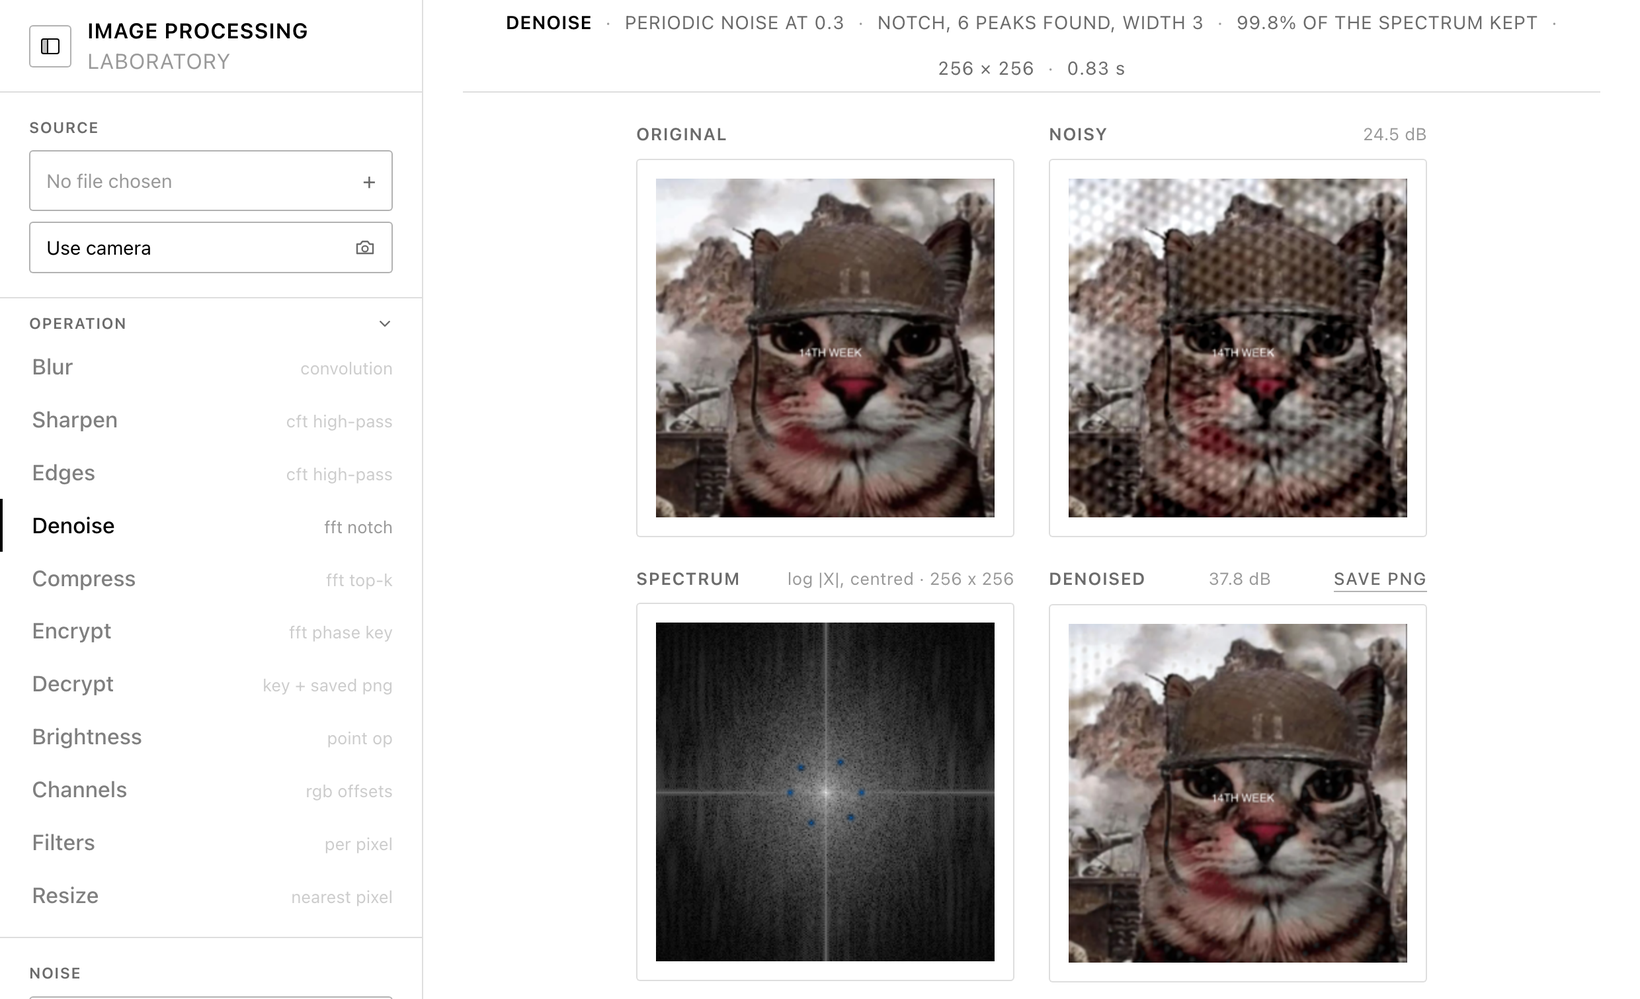
\includegraphics[width=\linewidth]{app_denoise}};}
\end{columns}
\end{frame}

%------------------------------------------------
\begin{frame}{What it can do}
\centering
\op{grid_input}{Input}{your photo}\hfill
\op{grid_blur}{Blur}{convolution}\hfill
\op{grid_sharpen}{Sharpen}{CFT high-pass}\hfill
\op{grid_edges}{Edges}{CFT high-pass}\hfill
\op{grid_denoise}{Denoise}{FFT notch filter}\hfill
\op{grid_compress}{Compress}{FFT top-$k$}

\vspace{1.2em}
\op{grid_encrypt}{Encrypt}{random phase}\hfill
\op{grid_decrypt}{Decrypt}{inverse phase}\hfill
\op{grid_brightness}{Brightness}{gain}\hfill
\op{grid_channels}{Channels}{RGB offsets}\hfill
\op{grid_filters}{Filters}{per-pixel maps}\hfill
\op{grid_resize}{Resize}{sampling}
\end{frame}

%------------------------------------------------
\begin{frame}{Architecture}
\centering
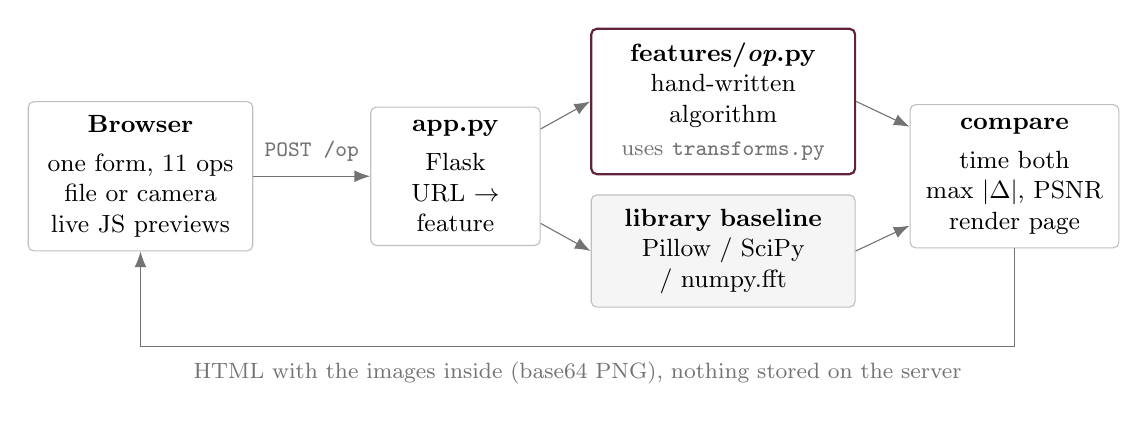
\begin{tikzpicture}[
    box/.style={draw=black!25, rounded corners=2pt, fill=white, align=center,
                font=\small, inner sep=5pt},
    ours/.style={box, draw=accent, thick},
    arr/.style={-{Latex[length=2mm]}, draw=black!55},
    lab/.style={font=\footnotesize, text=muted},
  ]
  \node[box, text width=2.5cm] (br) at (1.3,0)
    {\textbf{Browser}\\[3pt] one form, 11 ops\\ file or camera\\ live JS previews};
  \node[box, text width=1.8cm] (app) at (5.3,0)
    {\textbf{app.py}\\[3pt] Flask\\ URL $\to$ feature};
  \node[ours, text width=3.0cm] (hand) at (8.7,0.95)
    {\textbf{features/\emph{op}.py}\\ hand-written algorithm\\[1pt]
     {\footnotesize\color{muted}uses \texttt{transforms.py}}};
  \node[box, fill=black!4, text width=3.0cm] (lib) at (8.7,-0.95)
    {\textbf{library baseline}\\ Pillow / SciPy / numpy.fft};
  \node[box, text width=2.3cm] (out) at (12.4,0)
    {\textbf{compare}\\[3pt] time both\\ max $|\Delta|$, PSNR\\ render page};

  \draw[arr] (br) -- node[lab, above=2pt] {\texttt{POST /op}} (app);
  \draw[arr] (app) -- (hand.west);
  \draw[arr] (app) -- (lib.west);
  \draw[arr] (hand.east) -- (out);
  \draw[arr] (lib.east) -- (out);
  \draw[arr] (out.south) -- ++(0,-1.25) -| node[lab, pos=0.25, below=2pt]
    {HTML with the images inside (base64 PNG), nothing stored on the server} (br.south);
\end{tikzpicture}

\vspace{1.2em}
{\small\color{muted} Python 3.14 \enspace\textperiodcentered\enspace Flask
 \enspace\textperiodcentered\enspace NumPy (arithmetic only)
 \enspace\textperiodcentered\enspace Pillow, SciPy (baselines only)
 \enspace\textperiodcentered\enspace vanilla JS}
\end{frame}

%------------------------------------------------
\begin{frame}{Blur}
Each output pixel is a weighted average of its $k \times k$ neighbourhood.
The weights, the \alert{kernel}, decide the kind of blur.

\vspace{0.6em}
\begin{minipage}[c]{0.34\textwidth}\centering
  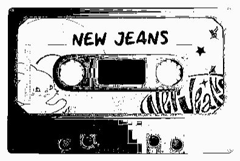
\includegraphics[width=\linewidth]{blur_input}\\[1pt]{\footnotesize\color{muted}input}
\end{minipage}\hfill
\begin{minipage}[c]{0.62\textwidth}\centering
  \kpair{box}{box}\hspace{14pt}\kpair{gaussian}{Gaussian}\\[4pt]
  \kpair{disk}{disc (lens)}\hspace{14pt}\kpair{motion}{motion 30\textdegree}
\end{minipage}

\vspace{1.2em}
\centering
{\small\color{muted} $9\times9$ kernels \enspace\textperiodcentered\enspace
 vs Pillow / SciPy: max $|\Delta| \le 1$ \enspace\textperiodcentered\enspace
 animated live in the browser}
\end{frame}

%------------------------------------------------
\begin{frame}[fragile,t]{Blur: theory}
\concept{LTI system \enspace\textperiodcentered\enspace impulse response \enspace\textperiodcentered\enspace 2D convolution}
\begin{columns}[T,totalwidth=\textwidth]
\column{0.41\textwidth}
Kernel $h$ = \textbf{impulse response}:
\[
  y[m,n] = \sum_{k}\sum_{l} h[k,l]\; x[m-k,\, n-l]
\]
\begin{itemize}
  \item Same weights everywhere: shift-invariant
  \item $\sum h = 1 \Rightarrow H(0,0) = 1$ (DC kept)
  \item Averaging $\Rightarrow$ \alert{low-pass} filter
\end{itemize}

\medskip
Gaussian: $h \propto e^{-(k^2+l^2)/2\sigma^2}$, \ $\sigma = \text{size}/6$

\medskip
{\small\color{muted} Edge pixels replicated at the border.\\
Cost $O(MNk^2)$: $11\times11$ at 500\,px $\approx 10$\,s.}

\column{0.55\textwidth}
\begin{lstlisting}
def convolve2d(x, h):
    h = h[::-1, ::-1]          # flip = convolution
    p = pad(x, K // 2, "edge") # replicate border
    for m in range(H):
        for n in range(W):
            s = 0.0
            for k in range(K):
                for l in range(K):
                    s += p[m+k, n+l] * h[k, l]
            y[m, n] = s
    return y                   # per colour channel

def gaussian_kernel(size):
    sigma = size / 6
    d = arange(size) - size // 2
    g = exp(-(d[:,None]**2 + d[None,:]**2)
            / (2 * sigma**2))
    return g / g.sum()         # sum(h) = 1
\end{lstlisting}
\end{columns}
\end{frame}

%------------------------------------------------
\begin{frame}{Resize}
Every new pixel copies the old pixel under its centre (nearest neighbour).
Nothing is averaged.

\vspace{0.8em}
\centering
\pic{1.8cm}{blur_input}{input}\hspace{3pt}
\pic{1.8cm}{resize_blocky}{$\times0.2$, then $\times5$}\hspace{16pt}
\pic{1.8cm}{zone}{zone plate}\hspace{3pt}
\pic{1.8cm}{zone_nearest}{$\downarrow 4$, nearest (ours)}\hspace{3pt}
\pic{1.8cm}{zone_lowpass}{$\downarrow 4$, low-pass first}

\vspace{0.8em}
\resizemap{3}{6}{1.4}{\textbf{Enlarge}\enspace $s = 3/6 = 0.5 < 1$}{every old pixel copied twice: blocky}%
\hspace{1.4cm}%
\resizemap{6}{4}{0.7}{\textbf{Shrink}\enspace $s = 6/4 = 1.5 > 1$}{pixels 1 and 4 never read: aliasing}

\vspace{0.8em}
{\small\color{muted} blocky when enlarged, false rings when shrunk
 \enspace\textperiodcentered\enspace identical to Pillow's NEAREST: max $|\Delta| = 0$}
\end{frame}

%------------------------------------------------
\begin{frame}[fragile,t]{Resize: theory}
\concept{sampling \enspace\textperiodcentered\enspace Nyquist
 \enspace\textperiodcentered\enspace aliasing \enspace\textperiodcentered\enspace zero-order hold}
\begin{columns}[T,totalwidth=\textwidth]
\column{0.41\textwidth}
Resizing resamples the image on a new grid, step $s = \text{old}/\text{new}$:
\[
  y[i] = x\bigl[\lfloor (i + \tfrac12)\, s \rfloor\bigr]
\]
\begin{itemize}
  \item \textbf{Shrink} ($s > 1$): frequencies above the new Nyquist
        $\tfrac{1}{2s}$ fold back: \alert{aliasing}
  \item Cure: low-pass \emph{before} sampling
  \item \textbf{Enlarge} ($s < 1$): each sample held,
        a zero-order hold: blocky
\end{itemize}

\column{0.55\textwidth}
\begin{lstlisting}
def old_positions(old, new):
    step = old / new
    pos = step / 2           # centre of pixel 0
    out = []
    for i in range(new):
        out.append(int(pos)) # old pixel below
        pos += step          # summed, as Pillow
    return out

def resize_nearest(img, scale):
    rows = old_positions(H, round(H * scale))
    cols = old_positions(W, round(W * scale))
    for y in range(len(rows)):
        for x in range(len(cols)):
            out[y, x] = img[rows[y], cols[x]]
    return out
\end{lstlisting}
\end{columns}
\end{frame}

%------------------------------------------------
\begin{frame}{Brightness, Channels \& Filters}
Each output pixel depends only on the same input pixel,
so the browser previews these \alert{live} while a slider moves.

\vspace{0.8em}
\centering
\pic{2.05cm}{grid_input}{input}\hspace{12pt}
\pic{2.05cm}{pt_brightness}{brightness $\times1.4$}\hspace{12pt}
\pic{2.05cm}{pt_channels}{R $+50$, B $-50$}\hspace{12pt}
\pic{2.05cm}{pt_grayscale}{grayscale}

\vspace{0.5em}
\pic{2.05cm}{pt_invert}{invert}\hspace{12pt}
\pic{2.05cm}{pt_bw}{black \& white}\hspace{12pt}
\pic{2.05cm}{pt_pixelate}{pixelate}\hspace{12pt}
\pic{2.05cm}{pt_vintage}{vintage}
\end{frame}

%------------------------------------------------
\begin{frame}[fragile,t]{Point operations: theory}
\concept{system properties \enspace\textperiodcentered\enspace memoryless
 \enspace\textperiodcentered\enspace linear vs non-linear}
\begin{columns}[T,totalwidth=\textwidth]
\column{0.54\textwidth}
Linear: $T\{a x_1 + b x_2\} = a\,T\{x_1\} + b\,T\{x_2\}$

\medskip
{\small
\begin{tabular}{@{}llcc@{}}
  \toprule
  System & $y$ & memoryless & linear \\
  \midrule
  Brightness     & $g\,x$                     & \checkmark & \checkmark \\
  Channels       & $x + d_c$                  & \checkmark & affine \\
  Gray, sepia    & $M\mathbf{x}$              & \checkmark & \checkmark \\
  Invert         & $255 - x$                  & \checkmark & affine \\
  Black \& white & $255\,[\text{luma} \ge T]$ & \checkmark & $\times$ \\
  Pixelate       & tile mean                  & $\times$   & \checkmark \\
  \bottomrule
\end{tabular}}

\medskip
{\small\color{muted} Clipping to $[0, 255]$ afterwards is itself a
non-linear system (saturation).}

\column{0.42\textwidth}
\begin{lstlisting}
for y in range(H):       # each pixel
    for x in range(W):   # on its own
        out[y, x] = f(img[y, x])

bright = lambda p: gain * p
shift  = lambda p: p + (dR, dG, dB)
gray   = lambda p: p + a*(luma(p) - p)
invert = lambda p: p + a*(255 - 2*p)
bw     = lambda p: 255 * (luma(p) >= T)

out = clip(out, 0, 255).astype(uint8)
\end{lstlisting}
\end{columns}
\end{frame}

%------------------------------------------------
\begin{frame}{Compress}
Keep only the strongest \alert{5\%} of the Fourier coefficients, store them compactly,
rebuild the image from them.

\vspace{1.2em}
\centering
\pic{3cm}{flower_input}{original \enspace 180.8 KB raw}\hspace{6pt}
\pic{3cm}{compress_mask}{bins kept}\hspace{6pt}
\pic{3cm}{compress_ours}{ours \enspace 22.4 KB \enspace 26.1 dB}\hspace{6pt}
\pic{3cm}{compress_jpeg}{JPEG \enspace 21.5 KB \enspace 42.9 dB}

\vspace{1.2em}
{\small\color{muted} 8.1$\times$ smaller than raw \enspace\textperiodcentered\enspace
 at the same size JPEG wins by 17 dB: it also quantises and entropy-codes}
\end{frame}

%------------------------------------------------
\begin{frame}[fragile,t]{Compress: theory}
\concept{energy compaction \enspace\textperiodcentered\enspace Parseval
 \enspace\textperiodcentered\enspace conjugate symmetry \enspace\textperiodcentered\enspace linearity}
\begin{columns}[T,totalwidth=\textwidth]
\column{0.41\textwidth}
Energy is the same in both domains (Parseval):
\[
  \sum_{m,n} |x[m,n]|^2 = \frac{1}{MN} \sum_{u,v} |X[u,v]|^2
\]
A photo's energy sits in few coefficients, so dropping the smallest $|X|$ costs little.

\bigskip
Real image $\Rightarrow$ \textbf{conjugate symmetry},
so one bin of each pair is enough:
\[
  X[-u,-v] = X^*[u,v]
\]

\bigskip
{\small\color{muted} Bins picked once, on luma (linearity).
14 bytes per stored pair.}

\column{0.55\textwidth}
\begin{lstlisting}
def encode(img, keep):
    X = [fft2(pad(img[c])) for c in RGB]
    L = .299*X[0] + .587*X[1] + .114*X[2]
    top = argpartition(abs(L), -k)[-k:]  # top k
    top = top | partner(top)     # whole pairs
    idx = one bin of each pair
    vals = float16(X[:, idx] / (M*N))  # 2 B
    return uint16(idx), vals

def decode(idx, vals):
    X = zeros((3, M, N), complex)
    X[:, idx] = vals * M*N
    X[:, partner(idx)] = conj(vals * M*N)
    return [ifft2(X[c]).real for c in RGB]
\end{lstlisting}
\end{columns}
\end{frame}

%------------------------------------------------
\begin{frame}{Denoise}
Stir periodic stripes into the photo, find them in the spectrum, cut them out.

\vspace{1.2em}
\centering
\pic{3cm}{cat_input}{clean}\hspace{6pt}
\pic{3cm}{denoise_noisy}{noisy \enspace 24.5 dB}\hspace{6pt}
\pic{3cm}{denoise_mask_zoom}{spectrum, 6 notches}\hspace{6pt}
\pic{3cm}{denoise_clean}{denoised \enspace \alert{37.8 dB}}

\vspace{1.2em}
{\small\color{muted} app defaults (stripes 30\%, notch width 3) \enspace\textperiodcentered\enspace
 99.8\% of the spectrum kept \enspace\textperiodcentered\enspace
 vs numpy.fft: max $|\Delta| = 0$}
\end{frame}

%------------------------------------------------
\begin{frame}[fragile,t]{The FFT, from scratch}
\concept{DFT \enspace\textperiodcentered\enspace Cooley--Tukey divide \& conquer
 \enspace\textperiodcentered\enspace $O(N\log N)$}
\begin{columns}[T,totalwidth=\textwidth]
\column{0.41\textwidth}
The DFT of $N$ samples:
\[
  X[k] = \sum_{n=0}^{N-1} x[n]\, W_N^{kn}, \quad W_N = e^{-j2\pi/N}
\]
Direct: $O(N^2)$. Split even ($E$) and odd ($O$):
\[
  \begin{aligned}
    X[k]              &= E[k] + W_N^k\, O[k] \\
    X[k+\tfrac{N}{2}] &= E[k] - W_N^k\, O[k]
  \end{aligned}
\]
$\log_2 N$ stages of butterflies: \alert{$O(N\log N)$}.

\bigskip
{\small\color{muted} $N = 1024$: DFT 148\,ms $\to$ FFT 1.2\,ms,
equal to numpy.fft within $10^{-12}$.\\[2pt]
Sides reflect-padded to $2^k$: a zero-padded edge is a step, which is broadband.}

\column{0.55\textwidth}
\begin{lstlisting}
def fft(x):                        # N = 2^m
    X = bit_reverse_order(x)
    for s in range(1, m + 1):      # log2 N stages
        M = 2**s
        wM = exp(-2j * pi / M)     # once per stage
        for l in range(0, N, M):   # each block
            w = 1
            for k in range(M // 2):     # butterflies
                a, b = l + k, l + k + M//2
                g, h = X[a], w * X[b]
                X[a], X[b] = g + h, g - h
                w *= wM
    return X

ifft = lambda X: conj(fft(conj(X))) / N  # reuse

fft2 = lambda a: fft_columns(fft_rows(a))  # separable
\end{lstlisting}
\end{columns}
\end{frame}

%------------------------------------------------
\begin{frame}[fragile,t]{Denoise: theory}
\concept{frequency response \enspace\textperiodcentered\enspace notch filter
 \enspace\textperiodcentered\enspace convolution theorem}
\begin{columns}[T,totalwidth=\textwidth]
\column{0.41\textwidth}
A sinusoid is \textbf{two spikes} in the spectrum:
\[
  \cos(2\pi\,\mathbf{k}_0 \!\cdot \mathbf{r})
  \;\longleftrightarrow\;
  \tfrac12\bigl[\delta(\mathbf{k}-\mathbf{k}_0) + \delta(\mathbf{k}+\mathbf{k}_0)\bigr]
\]
Filtering is multiplication in frequency:
\[
  Y[\mathbf{k}] = H[\mathbf{k}]\, X[\mathbf{k}]
  \;\Longleftrightarrow\; y = h * x
\]
Stripes sit far from the centre, the photo near it.
\alert{Notch} $H$: a small Gaussian hole at each spike.

\bigskip
{\small\color{muted} New here: the spectrum is centred (shift),
so low frequencies sit in the middle.}

\column{0.55\textwidth}
\begin{lstlisting}
X = shift(fft2(pad_reflect(luma(noisy))))
A = abs(X)
floor = 4 * quantile(A[outside centre], 0.999)

H = ones_like(A)
while A.max() > floor:           # hunt the spikes
    p = argmax(A)
    H *= 1 - exp(-dist(p)**2 / (2 * s**2))
    A[near p] = 0                # look for the next

for c in (R, G, B):              # same mask
    Xc = shift(fft2(pad_reflect(x[c])))
    y[c] = ifft2(unshift(Xc * H)).real[:h, :w]
\end{lstlisting}
\end{columns}
\end{frame}

%------------------------------------------------
\begin{frame}{Sharpen \& Edges}
Keep only the part of the image that changes fast.
Add it back: \alert{sharper}. Keep only its size: \alert{edges}.

\vspace{1.2em}
\centering
\pic{3cm}{sharpen_crop_before}{before}\hspace{6pt}
\pic{3cm}{sharpen_crop_after}{sharpened}\hspace{22pt}
\pic{3cm}{edges}{our edges}\hspace{6pt}
\pic{3cm}{edges_pillow}{Pillow FIND\_EDGES}

\vspace{1.2em}
{\small\color{muted} cutoff 15, amount 1.5 \enspace\textperiodcentered\enspace
 Pillow uses a different method (spatial kernels), so the two are compared by eye}
\end{frame}

%------------------------------------------------
\begin{frame}[fragile,t]{Sharpen \& Edges: theory}
\concept{continuous Fourier transform \enspace\textperiodcentered\enspace numerical integration
 \enspace\textperiodcentered\enspace high-pass filter}
\begin{columns}[T,totalwidth=\textwidth]
\column{0.41\textwidth}
Not the DFT here: the \textbf{continuous} FT of $f(x,y)$ on $[-1,1]^2$:
\[
  F(u,v) = \iint f(x,y)\, e^{-j2\pi(ux+vy)}\, dx\, dy
\]
evaluated by the \textbf{trapezoidal rule}, along $x$ then $y$.

\bigskip
Gaussian \alert{high-pass} ($D$ = distance from DC):
\[
  H(u,v) = 1 - e^{-D^2/2c^2}
\]
With $g = \mathcal{F}^{-1}\{H F\}$, the fine detail:\\[3pt]
\quad sharpen $= f + \alpha\, g$ \qquad edges $= |g|$

\column{0.55\textwidth}
\begin{lstlisting}
def cft(f, x, y, u, v):          # trapezoid rule
    for j in range(len(u)):      # along x, each u
        t = 2*pi*u[j]*x
        r1[:, j] = trapz(f * cos(t), x)
        r2[:, j] = trapz(f * sin(t), x)
    for i in range(len(v)):      # along y, each v
        c, s = cos(2*pi*v[i]*y), sin(2*pi*v[i]*y)
        re[i] =  trapz(r1*c - r2*s, y)
        im[i] = -trapz(r2*c + r1*s, y)
    return re, im

D = sqrt((u/du)**2 + (v/dv)**2)  # distance from DC
H = 1 - exp(-D**2 / (2 * c**2))  # Gaussian high-pass
detail = icft(re * H, im * H)

sharpened = f + amount * detail
edges = 1 - abs(detail) / abs(detail).max()
\end{lstlisting}
\end{columns}
\end{frame}

%------------------------------------------------
\begin{frame}{Encrypt \& Decrypt}
Scramble the phase of the spectrum with a passphrase.
The same passphrase unscrambles it; any other gives noise.

\vspace{1.2em}
\centering
\pic{3cm}{cat_input}{original}\hspace{6pt}
\pic{3cm}{encrypt_cipher}{ciphertext (a PNG)}\hspace{6pt}
\pic{3cm}{decrypt_right}{key \texttt{cse220} \enspace \alert{53.7 dB}}\hspace{6pt}
\pic{3cm}{decrypt_wrong}{key \texttt{cse221} \enspace 9.6 dB}

\vspace{1.2em}
{\small\color{muted} the PNG carries the scheme, stretch and crop inside it,
 so a saved ciphertext opens later with only the key}
\end{frame}

%------------------------------------------------
\begin{frame}[fragile,t]{Encrypt \& Decrypt: theory}
\concept{all-pass system \enspace\textperiodcentered\enspace phase vs magnitude
 \enspace\textperiodcentered\enspace invertible systems}
\begin{columns}[T,totalwidth=\textwidth]
\column{0.41\textwidth}
Multiply the spectrum by a unit-magnitude mask:
\[
  E = \mathcal{F}^{-1}\{\mathcal{F}\{x\}\, H\}, \quad H = e^{j\varphi},\ |H| = 1
\]
\begin{itemize}
  \item \textbf{All-pass}: energy unchanged
  \item Phase holds structure: scrambled
  \item $H^{-1} = H^* = e^{-j\varphi}$: \alert{exact} recovery
  \item Wrong key: $e^{j(\varphi-\varphi')}$, another scramble
\end{itemize}

\medskip
Odd phase, $\varphi[-u,-v] = -\varphi[u,v]$, keeps $E$ real, so it saves as a PNG.

\column{0.55\textwidth}
\begin{lstlisting}
def phase_mask(key, shape):
    r = rng(sha256(key)).random(shape)
    phi = pi * (r - mirror(r))    # odd phase
    return exp(1j * phi)          # |H| = 1

def encrypt(x, key):
    H = phase_mask(key, x.shape)
    E = ifft2(fft2(x) * H).real   # stays real
    return to_png(E)              # + scheme, crop

def decrypt(E, key):
    H = phase_mask(key, E.shape)
    return ifft2(fft2(E) * conj(H)).real
\end{lstlisting}
\end{columns}
\end{frame}

%------------------------------------------------
\begin{frame}{Results: ours vs the library}
\centering
{\small
\begin{tabular}{@{}llrrrr@{}}
  \toprule
  Operation & Baseline & Size & Ours & Baseline & max $|\Delta|$ \\
  \midrule
  FFT, $N = 1024$  & direct DFT, numpy.fft & 1024          & 1.2 ms  & 148 ms  & $10^{-12}$ \\
  Blur, box $5\times5$ & Pillow BoxBlur    & 500$\times$500 & 2.05 s  & 1.1 ms  & 1 \\
  Denoise, notch   & numpy.fft             & 256$\times$256 & 0.83 s  & 2.5 ms  & 0 \\
  Encrypt, phase   & numpy.fft             & 256$\times$256 & 0.71 s  & 3.7 ms  & 0 \\
  Brightness $\times1.4$ & ImageEnhance    & 500$\times$500 & 60 ms   & 0.26 ms & 1 \\
  Channels         & Image.point (LUT)     & 500$\times$500 & 60 ms   & 0.26 ms & 0 \\
  Grayscale        & Image.blend           & 500$\times$500 & 208 ms  & 0.14 ms & 1 \\
  Resize 50\%      & resize(NEAREST)       & 500$\times$500 & 8.5 ms  & 0.04 ms & 0 \\
  \bottomrule
\end{tabular}}

\vspace{1.2em}
\alert{Same answers} (within 1 grey level: rounding vs truncation),
\alert{190--1900$\times$ slower}: pure-Python loops against C.

\vspace{0.4em}
{\small\color{muted} Sharpen, edges and compress use a different method from their
baselines, so they are compared by eye and PSNR instead.}
\end{frame}

%------------------------------------------------
\begin{frame}[standout]
Thank you

\vspace{0.6em}
{\normalsize\mdseries Questions?}
\end{frame}

%================================================
\end{document}
